% Intended LaTeX compiler: xelatex
\documentclass[10pt, svgnames]{beamer}
\usepackage{graphicx}
\usepackage{longtable}
\usepackage{wrapfig}
\usepackage{rotating}
\usepackage[normalem]{ulem}
\usepackage{amsmath}
\usepackage{amssymb}
\usepackage{capt-of}
\usepackage{hyperref}
\usetheme{focus}
\author{Sappinandana Akamphon}
\date{\today}
\title{Analysis of Members under Combined Loadings}
\subtitle{ME 210: Mechanics of Materials}
\usepackage{booktabs}
\institute{Department of Mechanical Engineering, TSE}
\date{}
\usetikzlibrary{patterns,shapes,arrows,calc,decorations,decorations.markings,decorations.pathmorphing,patterns}
\AtBeginSection[]{\begin{frame}{Outline}\tableofcontents[currentsection]\end{frame}}
\usetikzlibrary{arrows,calc,decorations,decorations.markings,shapes,decorations.pathmorphing,patterns}
\pgfkeys{/tikz/.cd, view angle/.initial=0, view angle/.store in=\picangle}
\tikzset{horizontal/.style={y={(0,sin(\picangle))}},vertical at/.style={x={([horizontal] #1:1)}, y={(0,cos(\picangle)cm)}},every label/.style={font=, inner sep=1pt},shorten/.style={shorten <=#1, shorten >=#1},shorten/.default=3pt,->-/.style={decoration={markings, mark=at position #1 with {\arrow{>}}}, postaction={decorate}},->-/.default=0.5}
\hypersetup{
 pdfauthor={Sappinandana Akamphon},
 pdftitle={Analysis of Members under Combined Loadings},
 pdfkeywords={},
 pdfsubject={},
 pdfcreator={Emacs 30.0.50 (Org mode 9.6.1)}, 
 pdflang={English}}
\usepackage{biblatex}

\begin{document}


\begin{frame}[label={sec:orgfb04458}]{\{\}}
\maketitle
\end{frame}

\section{Pressure Vessels}
\label{sec:org0122df3}

\begin{frame}[label={sec:orgfaea732}]{Spherical Pressure Vessels}
\begin{columns}
\begin{column}{0.5\columnwidth}
\begin{center}
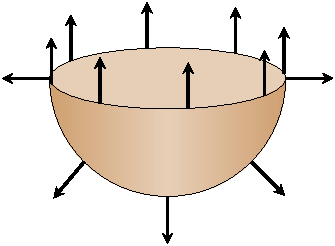
\includegraphics[height=0.4\textheight]{pictures/sphere-pressure-vessel.pdf}
\end{center}
\end{column}

\begin{column}{0.5\columnwidth}
$$ F_{\sigma} = F_p $$
$$ \sigma_2 \left( 2\pi r t \right) = p \pi r^2 $$
$$ \sigma_2 = \frac{pr}{2t} $$

\begin{itemize}
\item What about \(\sigma_1\)? How do you draw a Mohr's circle to represent state of stress?
\end{itemize}
\end{column}
\end{columns}
\end{frame}

\begin{frame}[label={sec:orgfd133c1}]{State of Stress of of Vessel Wall}
\begin{center}
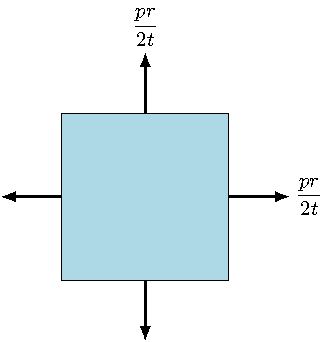
\includegraphics[height=0.8\textheight]{pictures/state-of-stress-spherical.pdf}
\end{center}
\end{frame}

\begin{frame}[label={sec:org28118e7}]{Mohr's Circle of State of Stress}
\begin{center}
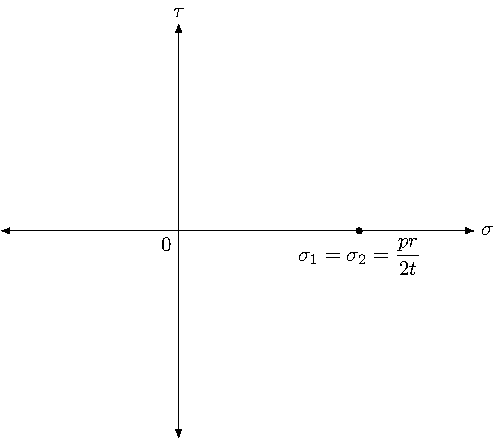
\includegraphics[height=0.8\textheight]{pictures/mohrs-sphere-vessel.pdf}
\end{center}
\end{frame}

\begin{frame}[label={sec:orgb332571}]{Absolute Maximum Shear Stress of Spherical Pressure Vessel}
\begin{center}
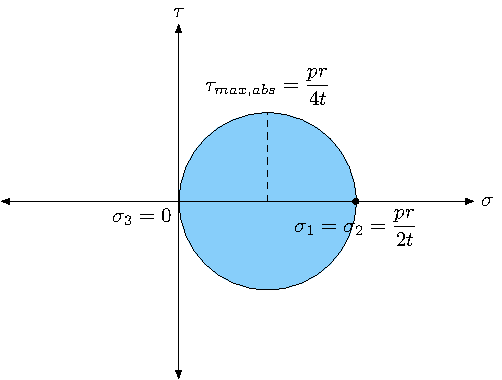
\includegraphics[height=0.8\textheight]{pictures/abs-max-shear-sphere-vessel.pdf}
\end{center}
\end{frame}

\begin{frame}[label={sec:orgbe0e966}]{Spherical Pressure Vessel: Summary}
\begin{itemize}
\item \(\sigma_1 = \sigma_2 = \dfrac{pr}{2t}\)
\item \(\tau_{xy} = \tau_{max} = 0\)
\item \(\tau_{max,abs} = \dfrac{pr}{4t}\)
\end{itemize}
\end{frame}

\begin{frame}[label={sec:orgdf7c407}]{Cylindrical Pressure Vessels}
\begin{columns}
\begin{column}{0.5\columnwidth}
\begin{center}
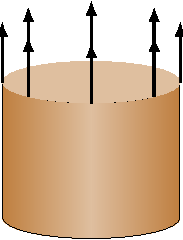
\includegraphics[width=.9\linewidth]{pictures/cylind-press-vess.pdf}
\end{center}
\end{column}

\begin{column}{0.5\columnwidth}
$$ F_{\sigma} = F_p $$
$$ \sigma_1 \left( 2tdy \right) = p \left( 2rdy \right) $$
$$ \sigma_1 = \frac{pr}{t} $$

$$ \sigma_2 \left( 2\pi rt \right) = p \pi r^2 $$
$$ \sigma_2 = \frac{pr}{2t} $$
\end{column}
\end{columns}
\end{frame}

\begin{frame}[label={sec:org17ccddf}]{State of Stress of of Vessel Wall}
\begin{center}
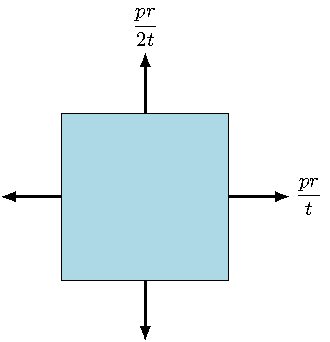
\includegraphics[height=0.8\textheight]{pictures/state-of-stress-cyl.pdf}
\end{center}
\end{frame}

\begin{frame}[label={sec:org3959c47}]{Mohr's Circle of Cylindrical Vessel}
\begin{center}
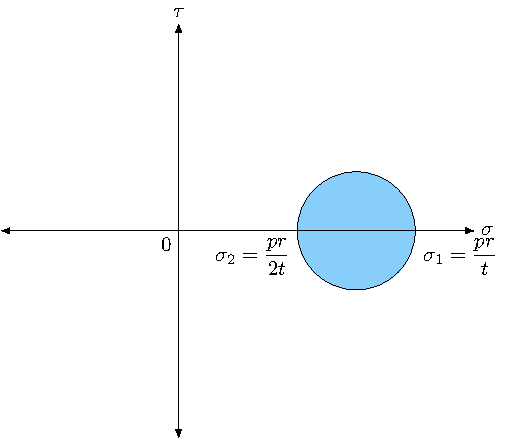
\includegraphics[height=0.8\textheight]{pictures/mohrs-cyl-vessel.pdf}
\end{center}
\end{frame}

\begin{frame}[label={sec:org9eaf518}]{Absolute Maximum Shear Stress of Cylindrical Vessel}
\begin{center}
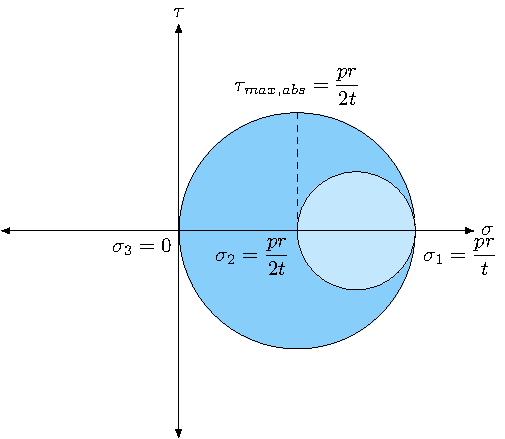
\includegraphics[height=0.8\textheight]{pictures/abs-max-shear-cyl-vessel.pdf}
\end{center}
\end{frame}

\begin{frame}[label={sec:org1b727a1}]{Cylindrical Pressure Vessel: Summary}
\begin{itemize}
\item \(\sigma_1 = \sigma_c = \dfrac{pr}{t}\)
\item \(\sigma_2 = \sigma_l = \dfrac{pr}{2t}\)
\item \(\tau_{xy} = 0, \tau_{max} = \dfrac{pr}{4t}\)
\item \(\tau_{max,abs} = \dfrac{pr}{2t}\)
\end{itemize}
\end{frame}

\begin{frame}[label={sec:org10441a0}]{Cylindrical Pressure Vessels}
\begin{itemize}
\item Failure of a shotgun barrel
\end{itemize}

\begin{center}
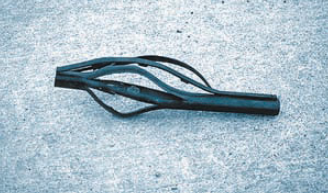
\includegraphics[width=.9\linewidth]{./pictures/shotgun-barrel.png}
\end{center}
\end{frame}

\section{Combined Loadings}
\label{sec:org50413d4}

\begin{frame}[label={sec:org70072e4}]{Combined Loadings}
\begin{itemize}
\item Multiaxial stress conditions come from
\begin{itemize}
\item Simultaneous application of loads
\item Complex geometry of component
\end{itemize}
\item Superposition is always the key
\begin{itemize}
\item Find stress(es) from each load
\item combine resultant stresses using multiaxial stress analysis
\end{itemize}
\end{itemize}
\end{frame}

\begin{frame}[label={sec:org3b03178}]{Design of Member under Combined Loadings}
\begin{itemize}
\item We need to know where failure starts
\item For a single-material component, failure starts where \emph{combined}
\end{itemize}
stress is the highest
\begin{itemize}
\item This is called the ``critical point''
\end{itemize}
\end{frame}

\begin{frame}[label={sec:org307f207}]{How to Identify the Critical Point}
\begin{itemize}
\item Identify each type of load (axial, bending, or torsion)
\item Mark locations of maximum stress for each load
\item Locate location(s) with multiple maximum stresses
\end{itemize}
\end{frame}


\begin{frame}[label={sec:org5b6a30d}]{Example: Helicoptor Rotor Shaft}
We want to determine the proper diameter of a rotor shaft for a 4-ton helicopter. The shaft is connected to the engine that provides the maximum torque of 8000 N-m. The shaft is made of AISI1023 steel with \(\sigma_{allow}\) = 400 MPa.

\begin{center}
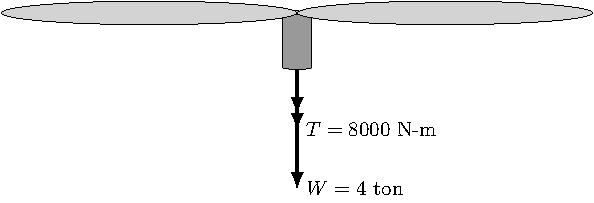
\includegraphics[width=.9\linewidth]{pictures/helicopter-example.pdf}
\end{center}
\end{frame}

\begin{frame}[label={sec:org893c7a0}]{Helicopter Rotor Shaft: Solution}
\begin{itemize}
\item Determine the critical point
\item Determine state of stress
\item Find proper radius \(r\)
\end{itemize}
\end{frame}

\begin{frame}[label={sec:org638be27}]{Helicopter Rotor Shaft: Solution}
\begin{align*}
  \sigma &= \frac{F}{A} = \frac{4(1000 \text{ kg/ton})(10 \text{ N/kg})}{\pi r^2} \\
         &= \frac{12732}{r^2} \\
  \tau &= \frac{Tr}{J} = \frac{8000(r)}{\pi r^4/2} \\
         &= \frac{5093}{r^3}
\end{align*}
\end{frame}

\begin{frame}[label={sec:orge241a84}]{Helicopter Rotor Shaft: Solution}
So the state of stress at the critical surface is a combination of normal stress and shear stress. Since the given material is limited by its normal stress, we need to determine the maximum principal stress.

\begin{align*}
\sigma_1 = \sigma_{allow} = 400 \times 10^6 &= \frac{12732}{2r^2} + \sqrt{ \left( \frac{12732}{2r^2} \right)^2 + \left( \frac{5093}{r^3} \right)^2 }
\end{align*}

This equation can be solved numerically to obtain \(r = 2.38\) cm.
\end{frame}

\begin{frame}[label={sec:org089a716}]{L-pipe}
\begin{center}
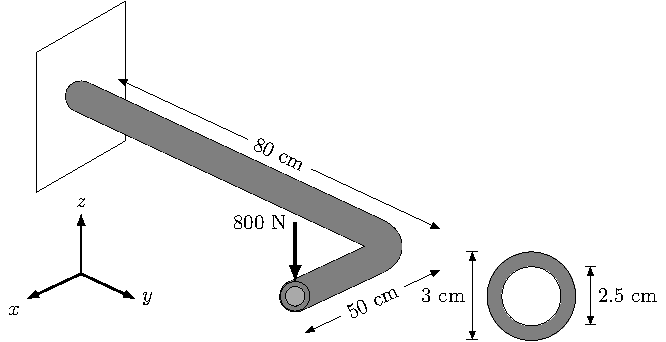
\includegraphics[width=.9\linewidth]{pictures/l-pipe.pdf}
\end{center}
\end{frame}

\begin{frame}[label={sec:orgf62b71a}]{Questions}
\begin{itemize}
\item Find the critical point. Elaborate your reasoning.
\item Determine the state of stress of the critical point.
\item Draw a Mohr's circle representing the state of stress.
\end{itemize}
\end{frame}
\end{document}